%------------------------------------------------------------------------------
% Author(s):
% Varaun Ramgoolie
% Copyright:
%  Copyright (C) 2020 Brad Bachu, Arjun Mohammed, Varaun Ramgoolie, Nicholas Sammy
%
%  This file is part of Applied-Mathematics-Unit2 and is distributed under the
%  terms of the MIT License. See the LICENSE file for details.
%
%  Description:
%     Year: 2016 
%     Module: 3
%     Question: 6 
%------------------------------------------------------------------------------

%------------------------------------------------------------------------------
% 6 a
%------------------------------------------------------------------------------

\begin{subquestions}
	
\subquestion
We are given a body which is being pulled up an inclined plane by a force.	

\begin{subsubquestions}
	
\subsubquestion
\textbf{\textit{Sketch and Translate:}} \\ \\
\begin{figure} [H]
	\begin{center}
		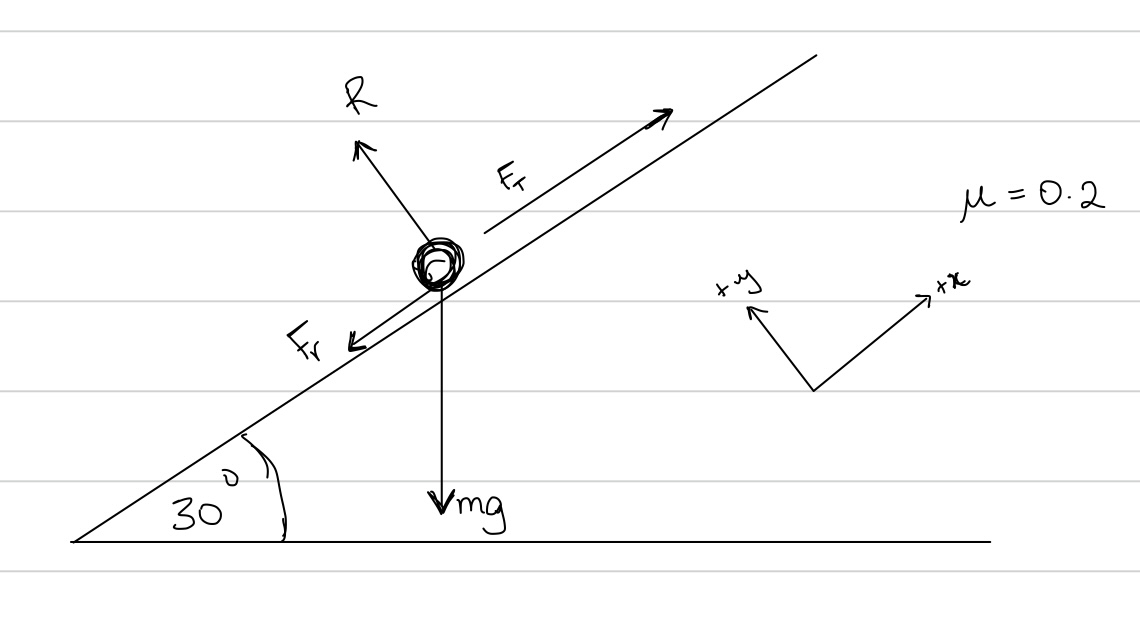
\includegraphics[scale=0.25]{../2016/figures/2016q6-1}
		\caption{\label{2016:q6:Sketch1} Body being pulled up the inclined plane.}
	\end{center}
\end{figure}
We are given the forces which act on the body and we also know that the body is moving at a constant speed. We want to find the tractive force acting parallel to the body and so, we should think about what we know about tractive force and how we can use the information given to us.	
	
	
	
	
\textbf{\textit{Simplify and Diagram:}} \\ \\
\begin{figure} [H]
	\begin{center}
		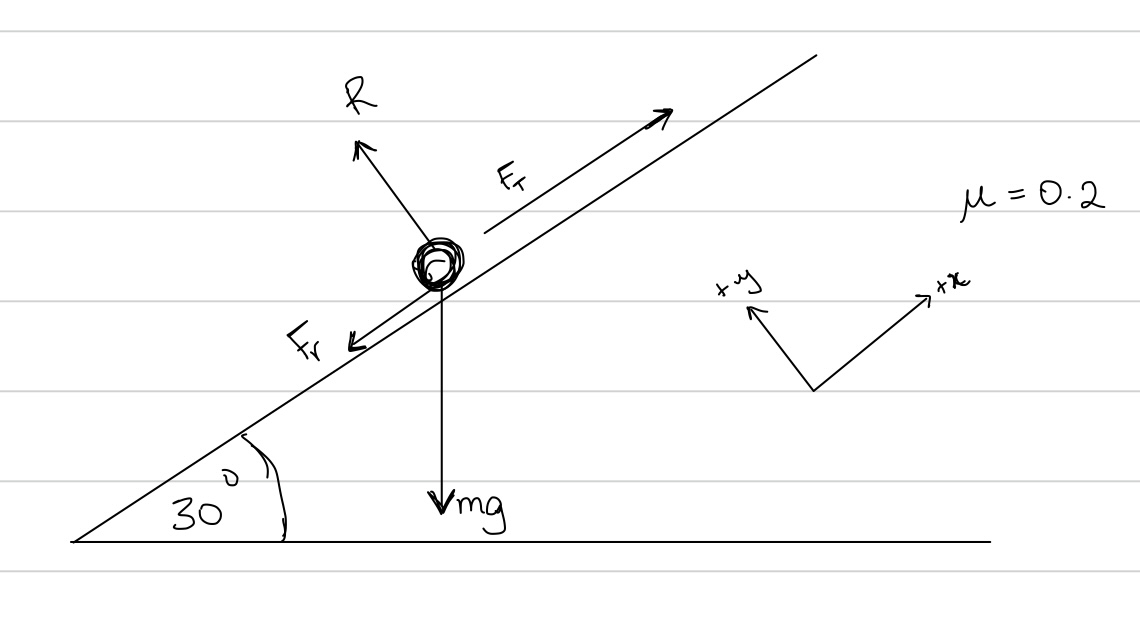
\includegraphics[scale=0.25]{../2016/figures/2016q6-1}
		\caption{\label{2016:q6:Diagram1} Free-body diagram of the body.}
	\end{center}
\end{figure}
We will first assume that the body acts as a point particle. From the fact that the body is moving at a constant speed, the acceleration (and by extension the Resultant Force acting on the body) must be 0. We have denoted the direction parallel to the plane as $x$ and the direction perpendicular to the plane as $y$. 
We will use,
\begin{itemize}
	\item $W$ to represent the weight of the particle acting downwards,
	\item $F_f$ to represent the frictional resistive force,
	\item $R$ to represent the normal reaction force of the particle on the plane,
	\item $F_T$ to represent the tractive force of the particle parallel to the plane.
\end{itemize}
To solve for the tractive force, we should use Newton's Second Law in the relevant directions of the particle.




\textbf{\textit{Represent Mathematically:}} \\ \\
Firstly, we should express the weight of the particle as its $x$ and $y$ components\footnote{This is exactly the same as resolving the force perpendicular and parallel to the plane.},
\begin{align}
	W & = -|W|\sin(30)\xhat - |W|\cos(30)\yhat \nn \\
	  & = -mg\sin(30)\xhat - mg\cos(30)\yhat \nn \\
\end{align}
	
If we apply Newton's Second Law to the system, we get that,
\begin{align}
	\sum \vec{F} & = m\vec{a} \nn \\
	& = m\vec{0} \nn \\
	\implies \sum F\xhat & = 0  \\
	& \text {and} \nn \\
	\sum F\yhat & = 0 \,.
\end{align}

Considering the forces in the $y$ direction, we see that,
\begin{equation}
	\sum F\yhat = R - mg\cos(30) = 0 \,. \label{2016:q6:REq1}
\end{equation}

Considering the forces in the $y$ direction, we see that,
\begin{align}
	\sum F\xhat & = F_T - mg\sin(30) -F_f = 0 \nn \\
	            \implies F_T & = mg\sin(30) + F_f \,. \label{2016:q6:EqnAi}
\end{align}




\textbf{\textit{Solve and Evaluate:}} \\ \\
From \req{2016:q6:REq1}, we can find that,
\begin{align}
	R - mg\cos(30) & = 0 \nn \\
	\implies R & = mg\cos(30) \,.
\end{align}

Therefore, our frictional force is,
\begin{align}
	F_f & = \mu R \nn \\
        & = \mu mg\cos(30) \,.
\end{align}

Finally, substituting $m=15$kg, $\mu=0.2$ and $g=10$ms$^{-2}$ into \req{2016:q6:EqnAi}, we get that,
\begin{align}
	F_T & = mg\sin(30) + F_f \nn \\
	    & = mg\sin(30) + \mu mg\cos(30) \nn \\
	    & = (15)(10)\left(\frac{1}{2}\right) + (0.2)(15)(10)\left(\frac{\sqrt{3}}{2}\right) \nn \\
	    & = 75 + 15\sqrt{3} \approx  100.98 N \,.
\end{align}

%------------------------------------------------------------------------------

\subsubquestion
\textbf{\textit{Simplify and Diagram:}} \\ \\
We want to find the work done moving the body up the plane after 1 second. We can consider the same diagram and assumptions from (a)(i). As we know that the body moves at a constant speed of 4ms$^{-1}$, the body will (by definition) move 4m up the plane after 1 second. Therefore, to find the work done, we can use our definition and equation for work and solve.




\textbf{\textit{Represent Mathematically:}} \\ \\
By definition, in order to move the body up the plane, we get that,
\begin{align}
\text{Work Done} & = F \times d \nn \\
                 & = F_T \times d \,.	\label{2016:q6:EqnAii}
\end{align}




\textbf{\textit{Solve and Evaluate:}} \\ \\
From \req{2016:q6:EqnAii}, we can substitute $d=4$m and $F_T=100.98$N and solve as,
\begin{align}
	\text{Work Done} & = F_T\times d \nn \\
	  & = 100.98\times 4 \nn \\
	  & \approx 404 J \,.
\end{align}

%------------------------------------------------------------------------------

\subsubquestion
\textbf{\textit{Simplify and Diagram:}} \\ \\
We want to find the power generated in part (a)(ii). We know that Power is the rate of doing work (with respect to time). Due to this definition, we can use the equation of Power and obtain our answer quite easily.




\textbf{\textit{Represent Mathematically:}} \\ \\
By definition, we know that,
\begin{equation}
	\text{Power} = \frac{\text{Work Done}}{\text{Time}} \,. \label{2016:q6:EqnAiii}
\end{equation}




\textbf{\textit{Solve and Evaluate:}} \\ \\
Substituting our values from part (a)(ii) into \req{2016:q6:EqnAiii}, we get that,
\begin{align}
	\text{Power} & = \frac{\text{Work Done}}{\text{Time}} \nn \\
				 & = \frac{404}{1} \nn \\
				 & = 404 W \,.
\end{align}

\end{subsubquestions}

%------------------------------------------------------------------------------
% 6 b
%------------------------------------------------------------------------------
	
\subquestion
We are given a particle being pulled along a rough horizontal plane.

\textbf{\textit{Sketch and Translate:}} \\ \\
\begin{figure} [H]
	\begin{center}
		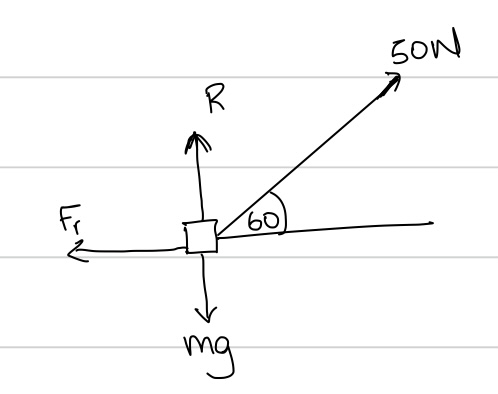
\includegraphics[scale=0.25]{../2016/figures/2016q6-2}
		\caption{\label{2016:q6:Sketch2} Body being pulled across the plane.}
	\end{center}
\end{figure}
We are given the forces which act on the body and we also know that the body is just about to move. We want to find the coefficient of friction of the surface. Therefore, we should think about how the forces interact with each other on the particle and what we know about friction




\textbf{\textit{Simplify and Diagram:}} \\ \\
\begin{figure} [H]
	\begin{center}
		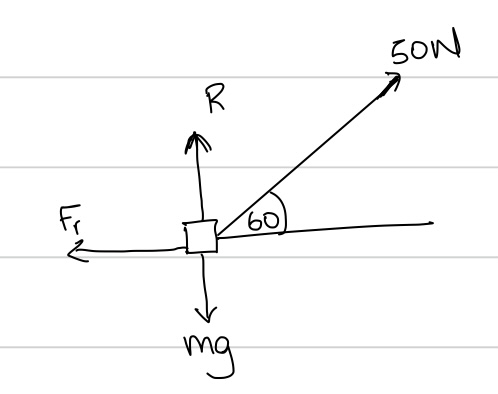
\includegraphics[scale=0.25]{../2016/figures/2016q6-2}
		\caption{\label{2016:q6:Diagram2} Free-body diagram of the particle.}
	\end{center}
\end{figure}
We will assume that the particle moves only on the horizontal plane. We will also assume that the forces act only in the $x$ and $y$ directions. as the particle is just about to slip, we know that the resultant force on the body is 0. Therefore, we can use Newton's Second Law and solve for the coefficient of friction.
We will use,
\begin{itemize}
	\item $W$ to represent the weight of the particle acting downwards,
	\item $F_f$ to represent the frictional resistive force,
	\item $R$ to represent the normal reaction force of the particle on the plane,
	\item $P$ to represent the 50N force pulling the particle.
\end{itemize}




\textbf{\textit{Represent Mathematically:}} \\ \\
Firstly, we should resolve the 50N force in the $x$ and $y$ directions as,
\begin{align}
	\vec{P} & = |P|\cos{60}\xhat + |P|\sin(60)\yhat \nn \\
	        & = |50|\cos{60}\xhat + |50|\sin(60)\yhat \nn \\
	         & = \left(50 \times \frac{1}{2}\right)\xhat + \left(50 \times \frac{\sqrt{3}}{2}\right)\yhat \nn \\
	         & = 25\xhat + 25\sqrt{3}\yhat \,.
\end{align}

If we apply Newton's Second Law to the system, we get that,
\begin{align}
	\sum \vec{F} & = m\vec{a} \nn \\
	& = m\vec{0} \nn \\
	\implies \sum F\xhat & = 0  \\
	& \text {and} \nn \\
	\sum F\yhat & = 0 \,.
\end{align}
	
Considering the forces in the $x$ direction,
\begin{align}
	\sum F\xhat & = 25 - F_f =0 \nn \\
	\implies F_f & = 25 \nn \\
	         \mu R & = 25 \,. \label{2016:q6:EqnB}
\end{align}

Considering the forces in the $y$ direction,
\begin{align}
	\sum F\yhat = R + 25\sqrt{3} -mg & = 0 \nn \\
	         \implies R & = mg - 25\sqrt{3} \,.
\end{align}




\textbf{\textit{Solve and Evaluate:}} \\ \\
By substituting $m=20$kg, $g=10$ms$^{-2}$, and $R = mg - 25\sqrt{3}$ into \req{2016:q6:EqnB}, we get,
\begin{align}
	\mu R & = 25 \nn \\
	\mu & = \frac{25}{R} \nn \\
	& = \frac{25}{mg - 25\sqrt{3}} \nn \\
	& = \frac{25}{200 - 25\sqrt{3}} \nn \\
	& \approx 0.16 \,.
\end{align}

%------------------------------------------------------------------------------
% 6 c
%------------------------------------------------------------------------------

\subquestion

\begin{subsubquestions}
	
\subsubquestion

We are given a situation where a collision occurs and the bodies become coupled after the collision.

\textbf{\textit{Sketch and Translate:}} \\ \\
\begin{figure}[H]
	\begin{center}
		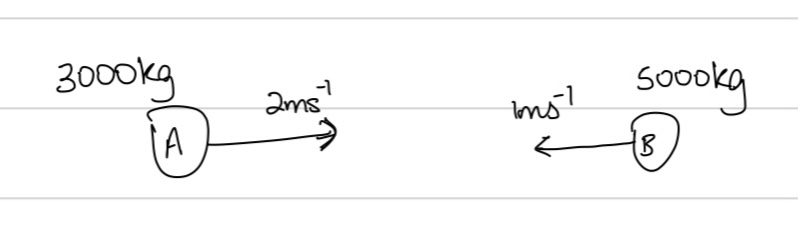
\includegraphics[scale=0.25]{../2016/figures/2016q6-3}
		\caption{\label{2016:q6:Sketch3} Bodies colliding with each other.}
	\end{center}
\end{figure}	
We are asked to find the velocity of B after impact. As we are given the mass and velocities of the bodies, we should begin thinking about what we know about their relationship and the momentum of the bodies.




\textbf{\textit{Simplify and Diagram:}} \\ \\
\begin{figure}[H]
	\begin{center}
		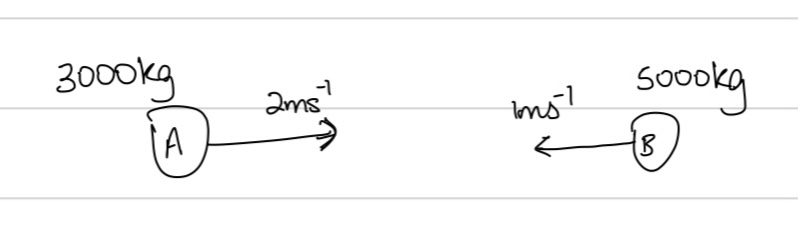
\includegraphics[scale=0.25]{../2016/figures/2016q6-3}
		\caption{\label{2016:q6:Diagram3} Collision overview with velocities and masses.}
	\end{center}
\end{figure}
We will assume that the collision occurs in a closed system (no external forces acting on the system). We will take movement to the right as positive and we will assume that the bodies only move in 1 dimension. We can use the Law of Conservation of Momentum to solve this problem.




\textbf{\textit{Represent Mathematically:}} \\ \\
From the Law of Conservation of Momentum, we get that,
\begin{align}
	\text{Total Momentum Before collision} & = \text{Total Momentum After collision} \nn \\
	m_1u_1 + m_2u_2 & = m_1v_1 + m_2v_2 \,.
\end{align}




\textbf{\textit{Solve and Evaluate:}} \\ \\
Substituting the values of $m_1=3000$kg, $m_2=5000$kg, $u_1=2$ms$^{-1}$, $u_2=-1$ms$^{-1}$ and $v_1=1.5$ms$^{-1}$, we get,
\begin{align}
	m_1u_1 + m_2u_2 & = m_1v_1 + m_2v_2 \nn \\
	(3000\times 2) + (5000\times -1) & = (3000\times 1.5) + 5000v_2 \nn \\
	6000-5000& = 4500 + 5000v_2 \nn \\
	\implies v_2 & = \frac{1000-4500}{5000} \nn \\
	             & = \frac{-7}{10} \text{ms}^{-1}
\end{align}
The speed of B is $\frac{7}{10}$ms$^{-1}$. 

%------------------------------------------------------------------------------

\subsubquestion

\textbf{\textit{Solve and Evaluate:}} \\ \\
The velocity of B is $\frac{-7}{10}$ms$^{-1}$. The negative sign indicates that B is moving to the left (as we took the positive direction as to the right).
	
%------------------------------------------------------------------------------

\subsubquestion

\textbf{\textit{Sketch and Translate:}} \\ \\
\begin{figure}[H]
	\begin{center}
		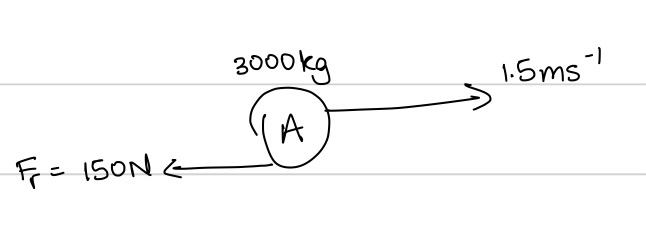
\includegraphics[scale=0.25]{../2016/figures/2016q6-4}
		\caption{\label{2016:q6:Sketch4} A after collision.}
	\end{center}
\end{figure}	
We are asked to find the time it takes for A to reach a stationary position. As we are given the frictional force acting on A, as well as the velocity of the particle afterwards. We can think about Newton's Second Law and its relationship with this system.
	
	
	
	
\textbf{\textit{Simplify and Diagram:}} \\ \\
\begin{figure}[H]
	\begin{center}
		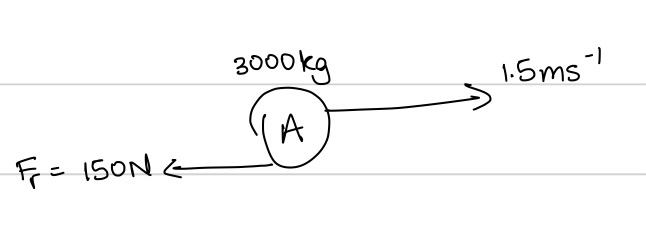
\includegraphics[scale=0.25]{../2016/figures/2016q6-4}
		\caption{\label{2016:q6:Diagram4} Free body diagram of A.}
	\end{center}
\end{figure}
We will take movement to the right as positive and we will assume that the body only move in 1 dimension. We will also assume that no external forces act in the plane of movement of the body except for friction, $F_f$ (which we assume is constant). Using Newton's Second Law, we can find the acceleration of the particle and use our equations of motion to solve for time.




\textbf{\textit{Represent Mathematically:}} \\ \\
Considering Newton's Second Law in the direction of motion, we know that,
\begin{align}
	\sum F & = ma \nn \\
	-F_f & = ma \nn \\
	a & = \frac{F_f}{m} \,.
\end{align}

Using this acceleration, we can solve for $t$ by using,
\begin{align}
	v & = u + at \nn \\
	\implies t & = \frac{v-u}{a} \,.
\end{align}




\textbf{\textit{Solve and Evaluate:}} \\ \\
Substituting $v=0$ms$^{-1}$, $u=1.5$ms$^{-1}$, $F_f=-150$N, $m=3000$kg and $a = \frac{F_f}{m}$, we get that\footnote{The value of $F_f$ is negative as the frictional force acts in the opposite direction of the motion of A.},
\begin{align}
	t & = \frac{v-u}{a} \nn \\
	  & = \frac{0-1.5}{\frac{F_f}{m}} \nn \\
	  & = \frac{-1.5}{\frac{-150}{3000}} \nn \\
	  & = 30s \,.
\end{align}

\end{subsubquestions}

\end{subquestions}


